% 
% file: sample.tex 
% author: Phil Rogaway
% History: 
%   Oct 14, 2003 - created
%   Apr 04, 2005 - last revised 
%
% This is LaTeX template to get you started using LaTeX
% for making problem-set solutions.
%
 
\documentclass[11pt]{article}
\usepackage{amsmath}
\usepackage{graphicx}
\usepackage{listings}
\setlength{\oddsidemargin}{0in}
\setlength{\evensidemargin}{0in}
\setlength{\textheight}{9in}
\setlength{\textwidth}{6.5in}
\setlength{\topmargin}{-0.5in}


%%%%%%%%%%%%%%%%%%%%%%%%%%%%%%%%%%%%%%%%%%%%%%%%%%%%%%%%%%%%%%%%%%%%%%%%%%%
\title{\bf Project\\[2ex] 
       \rm\normalsize ECS 256 --- Norm Matloff --- Winter 2014}
\date{\today}
\author{\bf }

\begin{document}
\maketitle


%%%%%%%%%%%%%%%%%%%%%%%%%%%%%%%%%%%%%%%%%%%%%%%%%%%%%%%%
\section*{Problem 1} 

As suggested by the hint, in order to find the bias at $t=0.5$, we're going to be examining the value of $\beta$ as n goes to $\infty$. The idea behind this is that the proposed model will converge to some $\beta$ as the number of samples increases, to the point that it fits as closely as possible to the actual function. Of course, it isn't possible for the model to fit precisely, because the actual relationship isn't linear like the model is, so there will be some bias in the resulting model. 

The first thing to consider is model construction. The simplest way to construct the model would be to use a least-squares method, so in the construction we would  minimize the following with respect to $g(X)$, which is the set of all possible functions for our model.

\begin{equation}
	E[(EY - g(X))^2]
\end{equation}•

For this problem, $g(X)=\beta X$ for all possible $\beta$, and the actual distribution of $EY$ is $X^{0.75}$, so we can rewrite this to minimizing the following with respect to $\beta$

\begin{equation}
	E[(X^{0.75} - \beta X)^2]
\end{equation}•

To actually find this value, we will first make a new variable $Q=(X^{0.75} - \beta X)^2$, and then use the continuous case of iterated expectations along X (eq 5.33) to find $EQ$

\begin{equation}
	EQ = \int _{-\infty} ^\infty f_X(t) \; E(Q | X = t)\; dt
\end{equation}•

\begin{equation}
	E(Q | X = t) = E[(t^{0.75} - \beta t)^2] = (t^{0.75} - \beta t)^2
\end{equation}•

X is $U(0,1)$, so $f_X(t)$ is 1 between the values of 0 and 1, and is zero elsewhere. With this and the value of $E(Q | X = t)$, we can rewrite $EQ$ as the following.

\begin{equation}
	EQ = \int _0 ^1 (t^{0.75} - \beta t)^2 \; dt
\end{equation}•

From here it's a simple matter to minimize with respect to $\beta$. First, finish computing the integral to get the final function of $\beta$ to minimize.

\begin{equation}
	EQ = \frac{1}{3}(\beta^2 - \frac{24}{11}\beta + \frac{6}{5})
\end{equation}•

And then take the derivative of the function with respect to $\beta$.

\begin{equation}
	\frac{d\,EQ}{d\beta} = \frac{2}{3}\beta - \frac{8}{11}
\end{equation}•

And finally set that equal to zero and solve for $\beta$, which yields $\beta=\frac{12}{11}$ as the value that minimizes our function.

Now we can move on and compute the bias. The bias is simply $\hat{m}_{Y;X}(t) - m_{Y;X}(t)$, which for the selected $\beta$ and $t=0.5$ is

\begin{equation}
	Bias(0.5) = \beta 0.5 - 0.5^{0.75} \approx {\fbox {\parbox{0.5in}{-0.0491}}}
\end{equation}•

%%%%%%%%%%%%%%%%%%%%%%%%%%%%%%%%%%%%%%%%%%%%%%%%%%%%

\section*{Problem 2}


\section*{Problem 3}
Our next data set explores house value in California. Kelley Pace and Ronald Barry used 1990 census data to divide California into geographic block groups with population 1425.5 persons on average. There are 20640 entries.

We are interested in how the following variables affect median house value: median income, housing median age, total rooms, total bedrooms, population, households, latitude, and longitude.

Here is R's summary output of the data:
\begin{verbatim}
Median.House.Value Median.Income       Median.Age   
 Min.   : 14999     Min.   : 0.4999   Min.   : 1.00  
 1st Qu.:119600     1st Qu.: 2.5634   1st Qu.:18.00  
 Median :179700     Median : 3.5348   Median :29.00  
 Mean   :206856     Mean   : 3.8707   Mean   :28.64  
 3rd Qu.:264725     3rd Qu.: 4.7432   3rd Qu.:37.00  
 Max.   :500001     Max.   :15.0001   Max.   :52.00
Total.Rooms    Total.Bedrooms     Population   
 Min.   :    2   Min.   :   1.0   Min.   :    3  
 1st Qu.: 1448   1st Qu.: 295.0   1st Qu.:  787  
 Median : 2127   Median : 435.0   Median : 1166  
 Mean   : 2636   Mean   : 537.9   Mean   : 1425  
 3rd Qu.: 3148   3rd Qu.: 647.0   3rd Qu.: 1725  
 Max.   :39320   Max.   :6445.0   Max.   :35682
 Households        Latitude       Longitude     
 Min.   :   1.0   Min.   :32.54   Min.   :-124.3  
 1st Qu.: 280.0   1st Qu.:33.93   1st Qu.:-121.8  
 Median : 409.0   Median :34.26   Median :-118.5  
 Mean   : 499.5   Mean   :35.63   Mean   :-119.6  
 3rd Qu.: 605.0   3rd Qu.:37.71   3rd Qu.:-118.0  
 Max.   :6082.0   Max.   :41.95   Max.   :-114.3  
 \end{verbatim}

 
 Next we use our Parsimony package on the data at various k levels. Here are the calls and output:
\begin{verbatim}
 > prsm(df[,1],df[,2:9],k=0.01, predacc=ar2, crit='max', printdel=T)
full outcome =  0.6369649 
deleted         Total.Rooms 
new outcome  =  0.6350863 
deleted         Total.Bedrooms 
new outcome  =  0.6321316 
[1] "Median.Income" "Median.Age"    "Population"    "Households"    "Latitude"      "Longitude"
\end{verbatim}
\begin{verbatim}
> prsm(df[,1],df[,2:9],k=0.05, predacc=ar2, crit='max', printdel=T)
full outcome =  0.6369649 
deleted         Median.Age 
new outcome  =  0.6243571 
deleted         Total.Rooms 
new outcome  =  0.6218261 
deleted         Total.Bedrooms 
new outcome  =  0.6198323 
[1] "Median.Income" "Population"    "Households"    "Latitude"      "Longitude"
 \end{verbatim}
By loosening our k value, the model selector decides to remove Median Age in the latter run. It is interesting to note that longitude and latitude remain in the model, which we will address later.

Next we want to compare our Parsimony package to the significance testing approach. 

Here is the summary of the coefficients of our lm() call in R:
\begin{verbatim}
Coefficients:
                 Estimate Std. Error t value Pr(>|t|)    
(Intercept)    -3.594e+06  6.254e+04 -57.468  < 2e-16 ***
Median.Income   4.025e+04  3.351e+02 120.123  < 2e-16 ***
Median.Age      1.156e+03  4.317e+01  26.787  < 2e-16 ***
Total.Rooms    -8.182e+00  7.881e-01 -10.381  < 2e-16 ***
Total.Bedrooms  1.134e+02  6.902e+00  16.432  < 2e-16 ***
Population     -3.854e+01  1.079e+00 -35.716  < 2e-16 ***
Households      4.831e+01  7.515e+00   6.429 1.32e-10 ***
Latitude       -4.258e+04  6.733e+02 -63.240  < 2e-16 ***
Longitude      -4.282e+04  7.130e+02 -60.061  < 2e-16 ***
--- 
\end{verbatim}
The significance testing approach would not delete any predictors. This data set has a large size (20640) so it makes sense that the predictors are all deemed significant.

Here is a summary of the comparison of methods:

\begin{tabular}{ | c | p{3cm} | p{3cm} | c  |}
\hline
Method&Parsimony (k=0.01) & Parsimony (k=0.05) & Significance Testing \\
\hline
Columns\newline Deleted& Total Rooms \newline Total Bedrooms & Total Rooms \newline Total Bedrooms \newline Median Age & None \\
\hline
Adjusted RSquared & 0.6321316 & 0.6218261 & 0.6369649 \\
\hline
\end{tabular}

Next we will discuss latitude and longitude. Looking at the full lm() summary above, latitude and longitude both have negative coefficient values. This says if we travel east or north, on average house value decreases. However using a model that says blocks at this longitude on average have the same house value seems crazy.  Blocks with similar longitudes aren't necessarily close in distance. In a large state like California there are expensive and inexpensive neighborhoods all over the state. 

So we will also remove latitude and longitude and make conclusions about the data. Here is the summary of the lm() call:
\begin{verbatim}
Coefficients:
                Estimate Std. Error t value Pr(>|t|)    
(Intercept)   -32165.268   2167.358  -14.84   <2e-16 ***
Median.Income  43094.918    284.263  151.60   <2e-16 ***
Median.Age      2000.544     45.080   44.38   <2e-16 ***
Population       -43.045      1.127  -38.20   <2e-16 ***
Households       152.700      3.344   45.66   <2e-16 ***
\end{verbatim}
First we see that income positively affects house value which is unsurprising. If people have more income, they can afford more expensive houses.

Next looking at age, we see it also positively affects house value. One would expect older people to have more money and this reflected in the high co-variance between these predictors.

Moving onto population, we see it negatively affects house value. With this data set each block has approximately similar geographic size, so blocks with higher population can be assumed to be denser. From our model we can conclude less dense areas have higher housing value. 

Finally we we look at households which positively affects house value. This is a bit surprising since population had a negative coefficient. 

Since we had coordinates, we decided to plot our data on a map of California using R's ggmap library. First we looked at a map of California as a whole, then zoomed into the Bay Area and the Greater Los Angeles area.

\newpage
\begin{figure}[H]
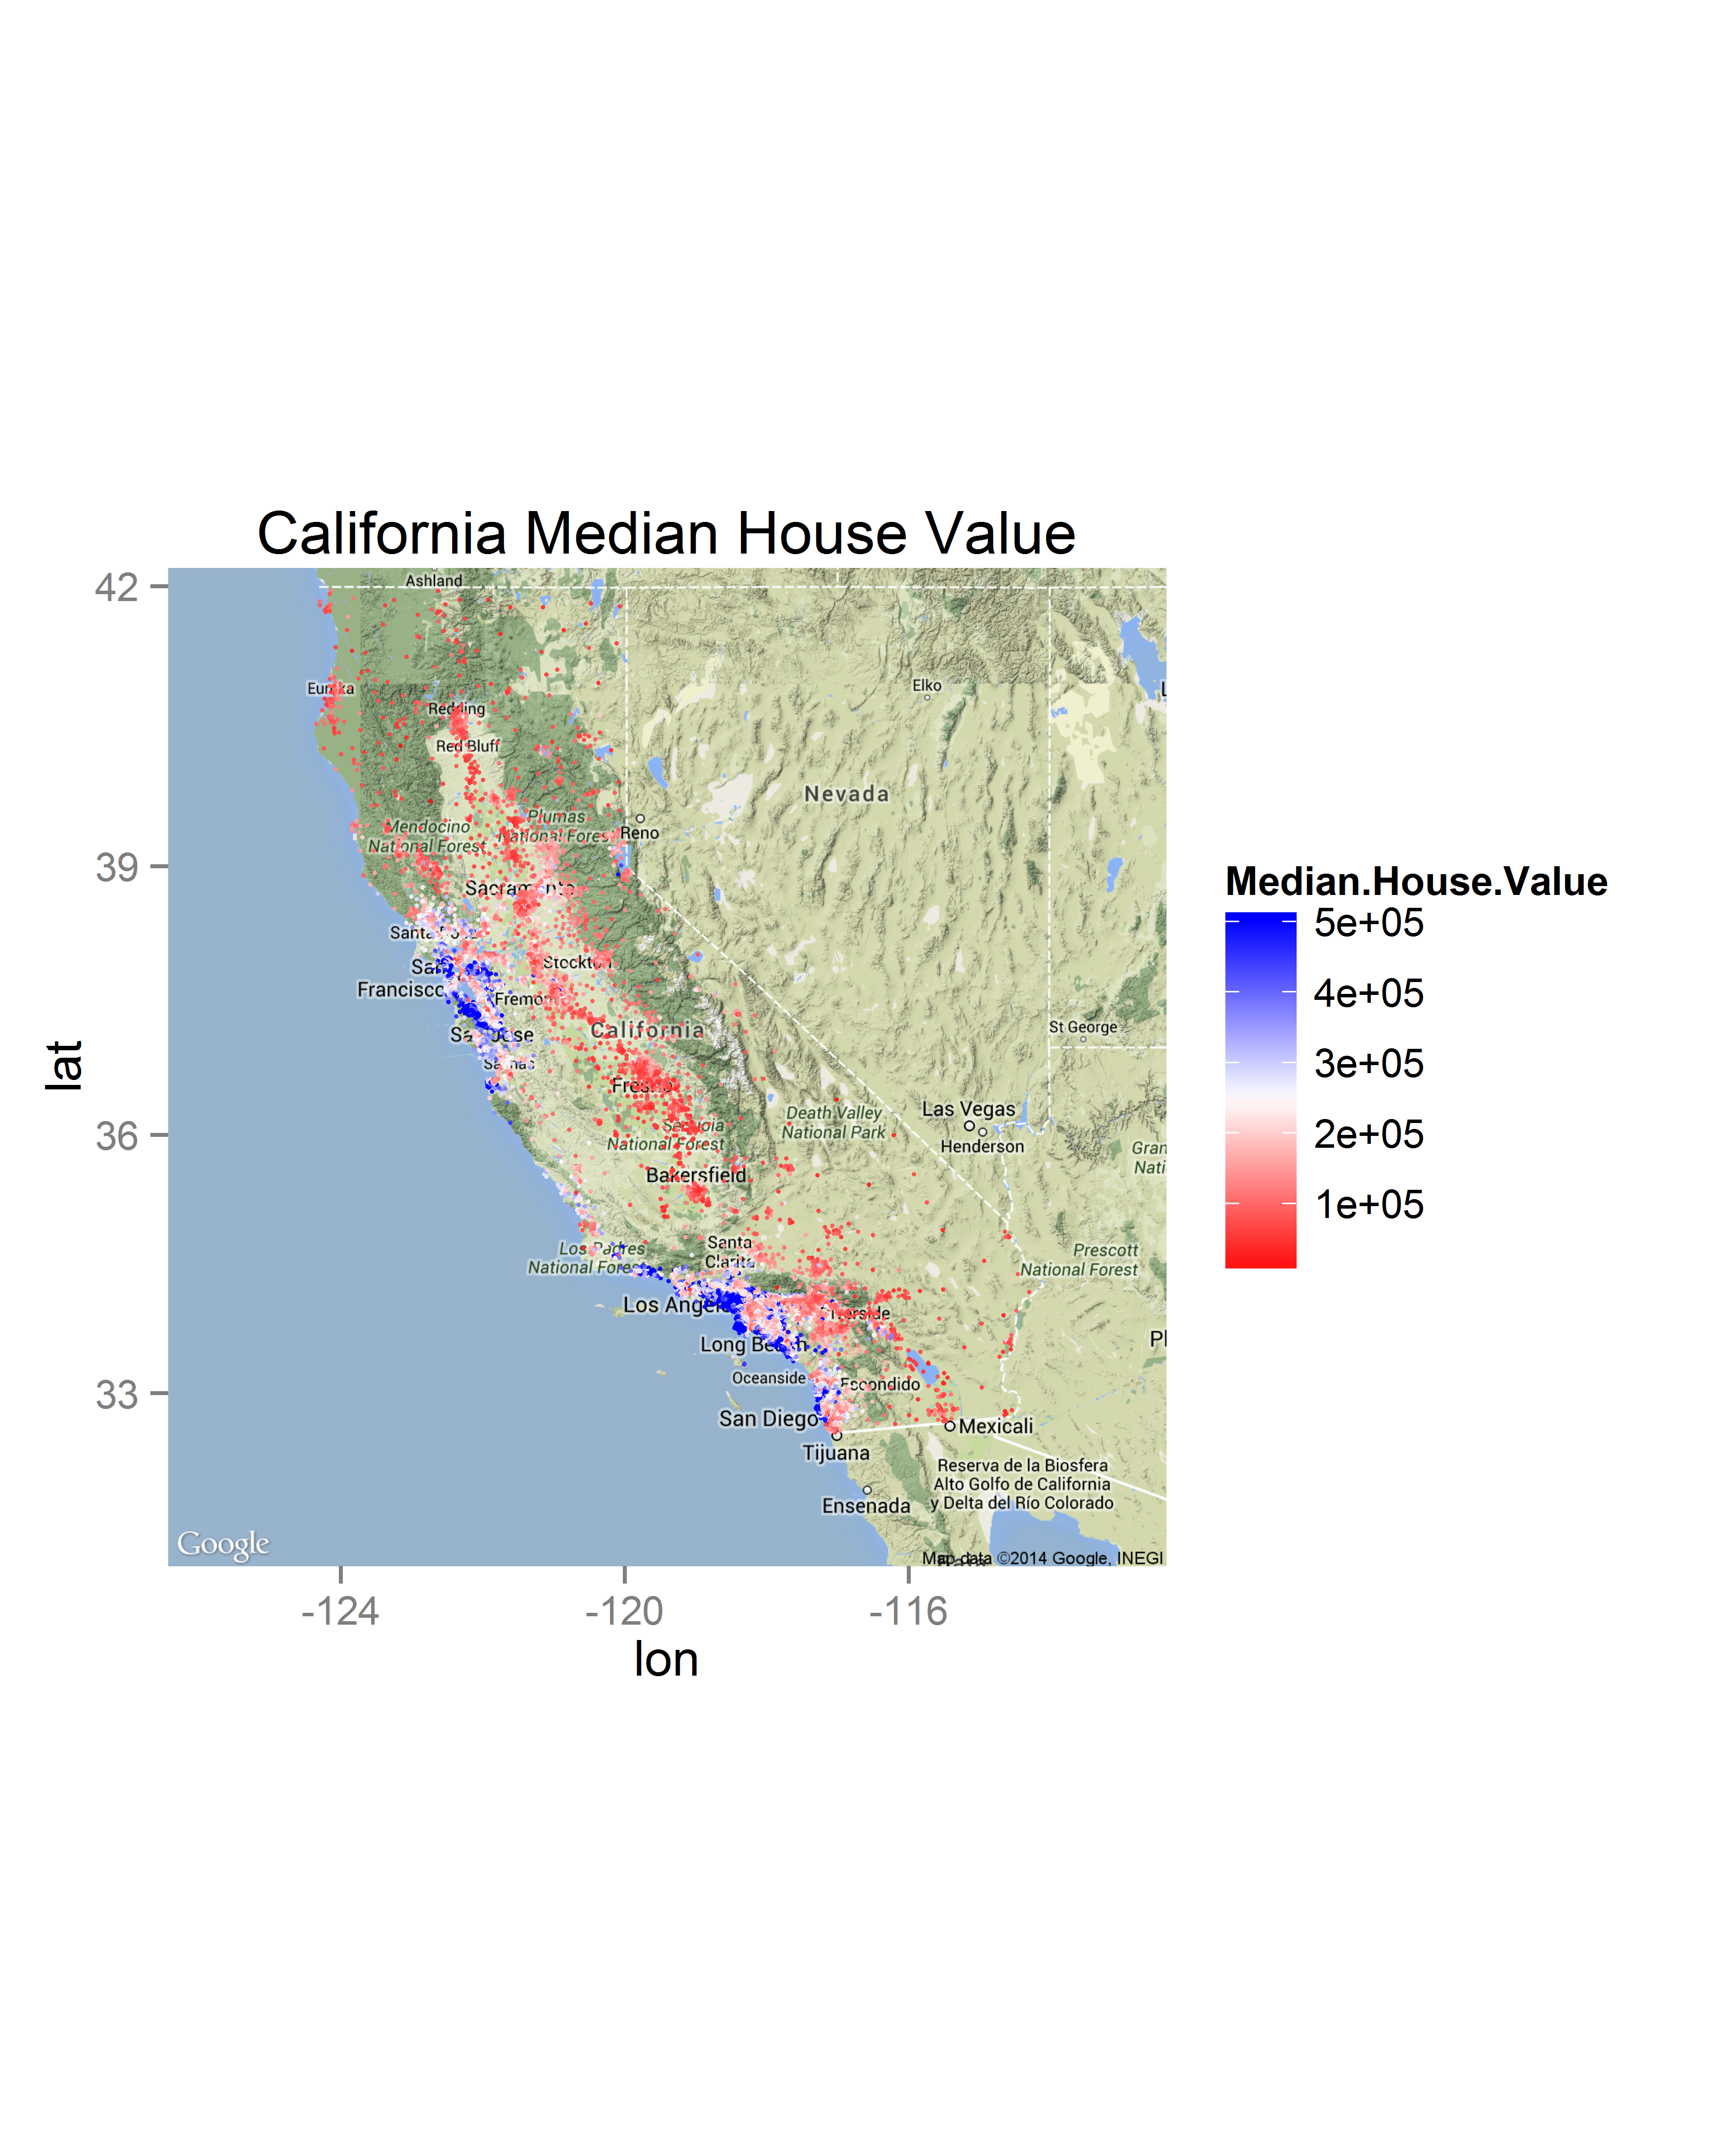
\includegraphics[scale=.54]{california.png}
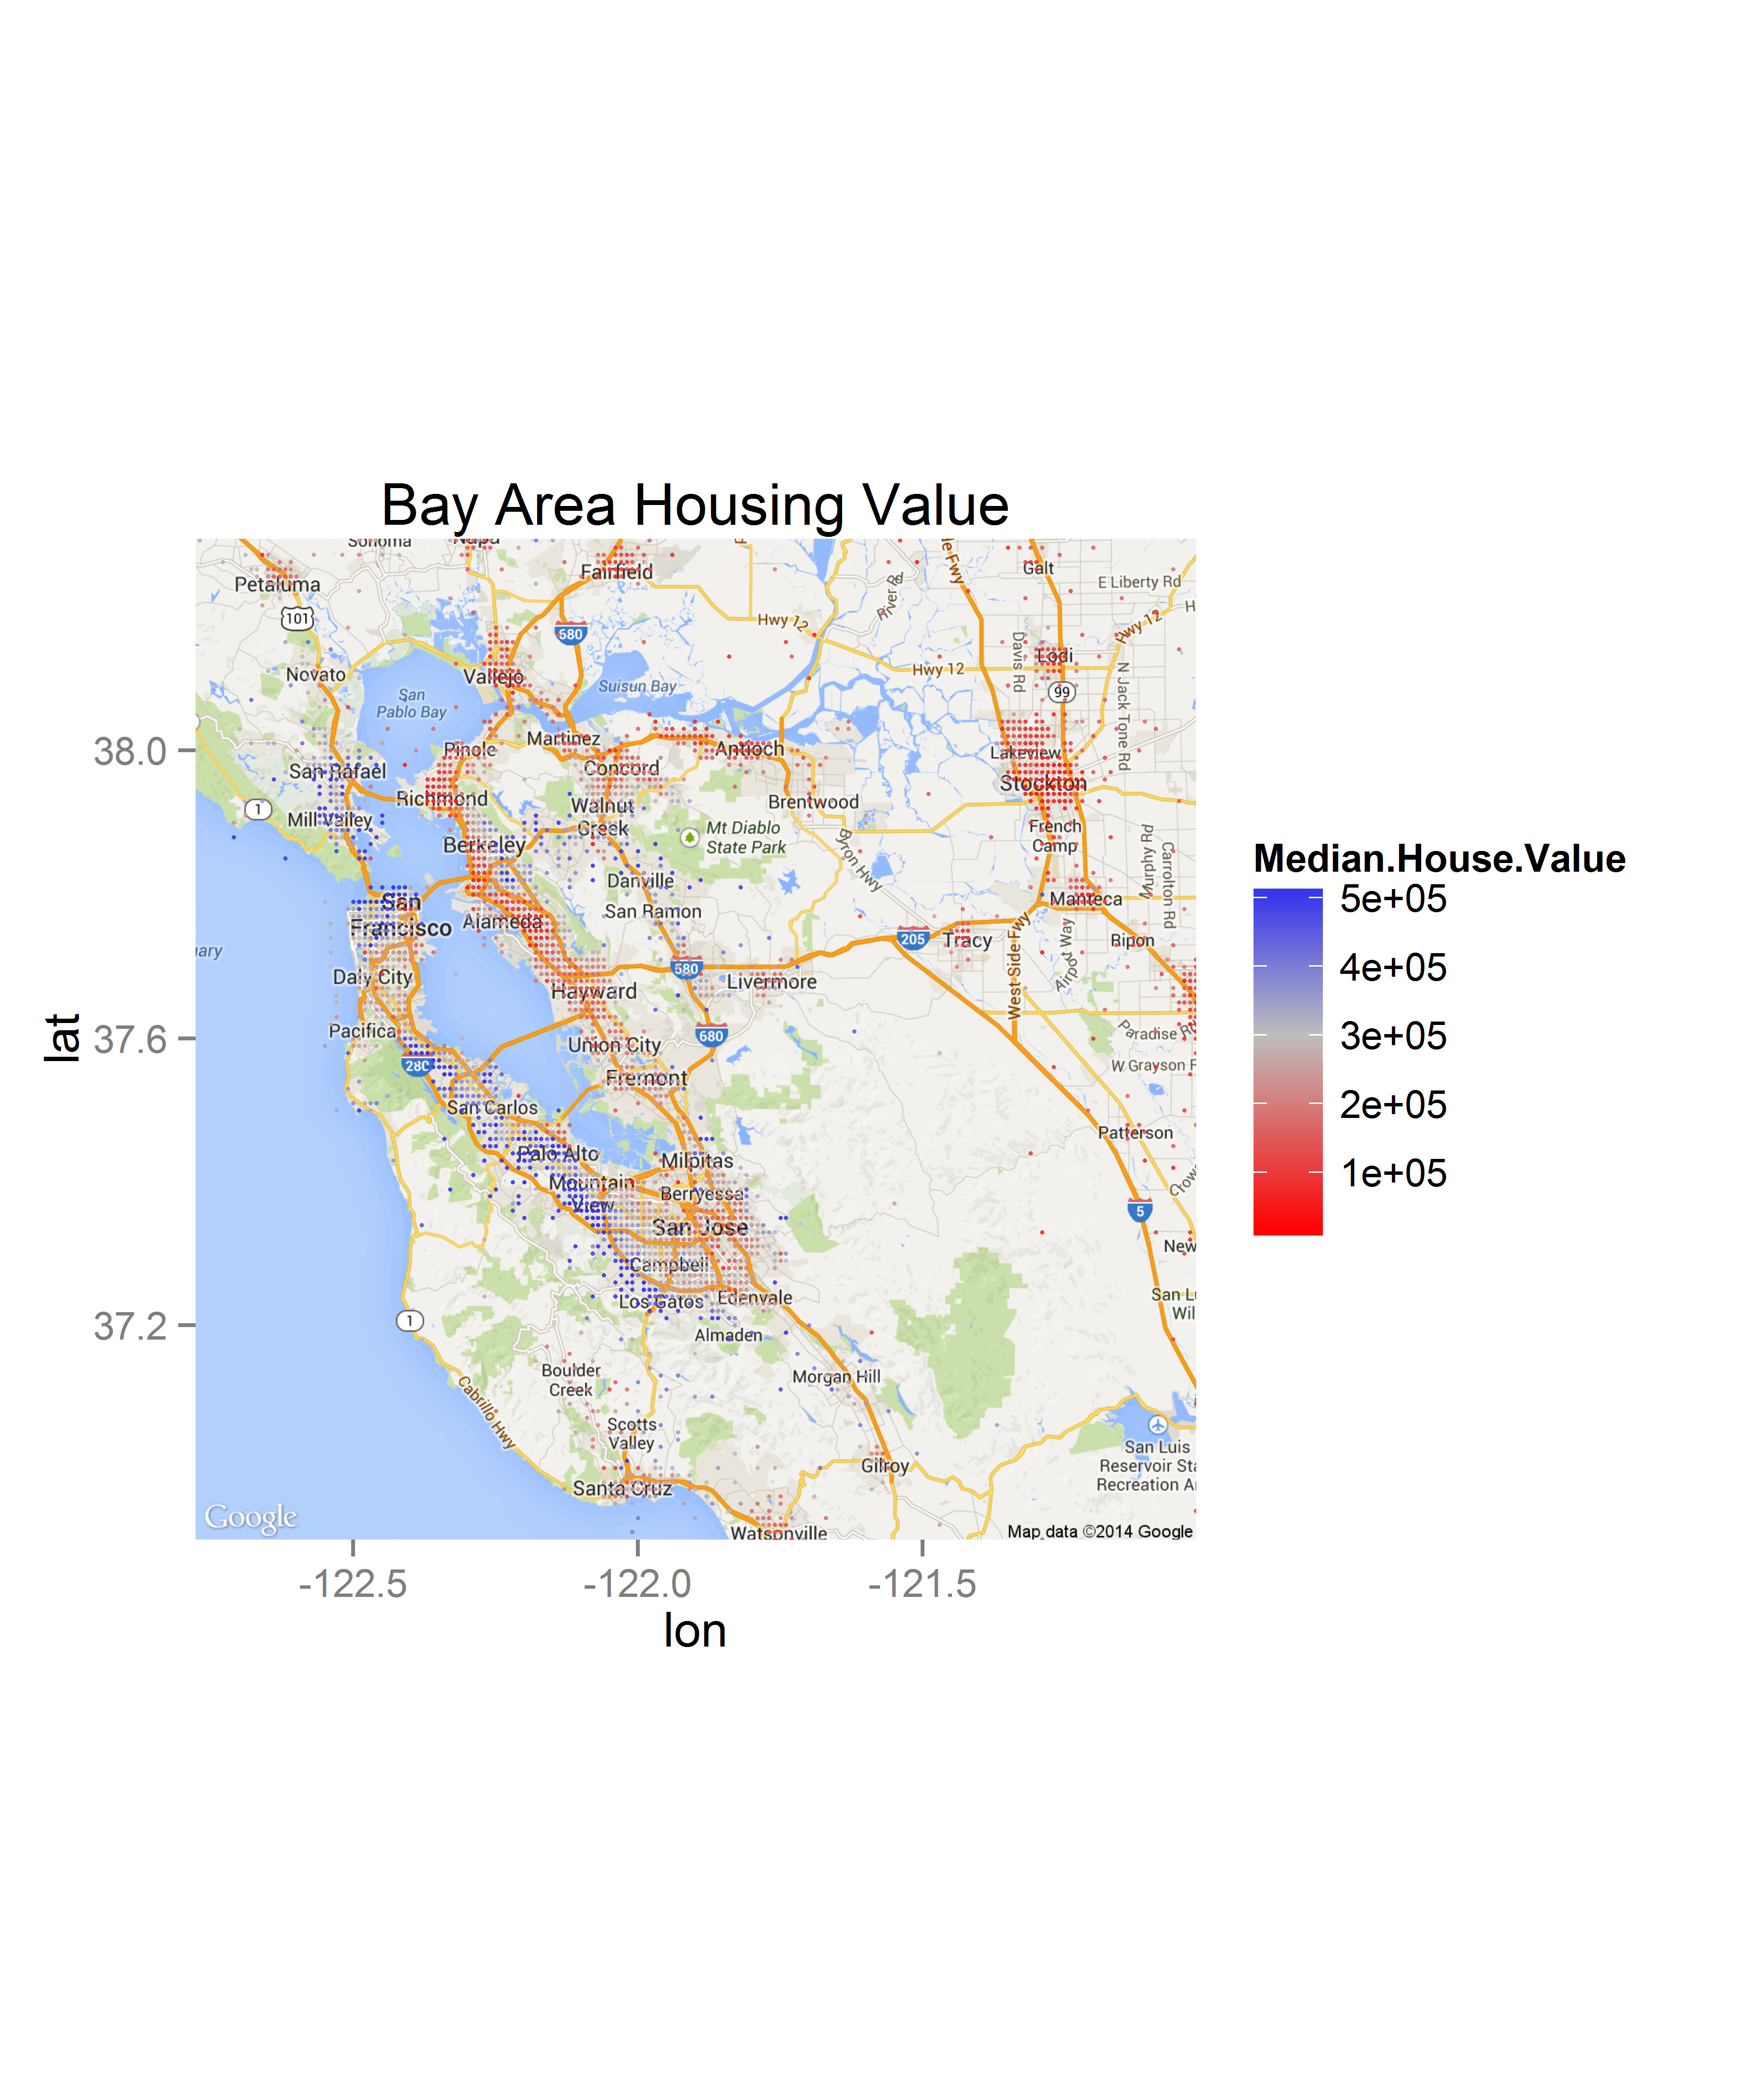
\includegraphics[scale=.54]{bayarea.png}
\includegraphics[scale=.7]{losangeles.png}
\end{figure}
The visualization helps us see how housing value is clustered in the state. As one might expect, rural areas generally have lower housing value than metropolitan areas. Within the metropolitan areas there are visible divisions as well.

\newpage
Next we looked at space shuttle data taken from the UCI Machine Learning Repository. The goal was to predict the class given 8 predictors, with 43500 data points. Our logistic regression predicted whether or not the class was of type 1.  The description of the data set was very poor, however it matched our criterion for dimension, data points, and regression type. Because of the lack of sufficient description, few conclusions can be drawn from the data, but we can test our Parsimony package just fine.

Here is the summary of results using Parsimony:

\begin{tabular}{ | c | p{3cm} | p{3.3cm} | c  |}
\hline
Method&Parsimony (k=0.01) & Parsimony (k=0.05) & Significance Testing \\
\hline
Columns Deleted& V1,V3,V4,V6,V9 & V1,V2,V3,V4,V6,V9 & V4 \\
\hline
AIC & 8575.803 & 8728.906 & 8475.2 \\
\hline
\end{tabular}


We also tested the various methods against a validation training set. We looked at the probability of correctly identifying a class 1 or not class 1. Also if we identified something as class 1, what was the probability it was actually class 1 and the same for not class 1.

Here is a summary of the results:

\begin{tabular}{ | c | p{3cm} | p{3.3cm} | c  |}
\hline
Method&Parsimony (k=0.01) & Parsimony (k=0.05) & Significance Testing \\
\hline
P(Correct ID $|$ class 1) & 0.9862345 & 0.9861474 & 0.9864959 \\
\hline
P(Correct ID $|$ not class 1) & 0.9285242 & 0.9285242 & 0.9169424 \\
\hline
P(Correct ID $|$ guess class 1) & 0.981276 & 0.9812744 & 0.9783135 \\
\hline
P(Correct ID $|$ guess not class 1) & 0.9466937 & 0.9463744 & 0.9470267  \\
\hline
\end{tabular}

The results for for the different methods are very close and it is hard to detect much difference in the accuracy levels. There were slightly fewer false positives and there was a slightly better detection of negatives for the Parsimony models. By simplifying the model, there is a possibility of increased accuracy during validation runs.
\end{document}
